The method was implemented in C++ using the \texttt{Eigen} library for linear algebra operations, particularly for the creation of the sparse matrix $\vf{A}$ described above and the resolution of the resulting linear system using the Cholesky decomposition. We did not make use of parallelization for simplicity, but the reader may note that if more accurate results are needed, using for example a denser grid around the boundary of the object, and thus increasing the size of the discrete domain, parallelization should be a must.

Implementing the numerical scheme outlined in Section \ref{sec: diffScheme}, we have the opportunity to explore the dynamics of fluid flow around various objects. \footnote{For further details on the implementation, we shared our code in the accompanying C++ code documentation. There the reader will also find animations of the flow dynamics around different objects to better understand the phenomenon.}
} First, we want to illustrate the emergence of the phenomenon, before delving in different factors on the flow as differences in Reynolds numbers or in the shape of the object.

\subsection{Observing Karman vortex street}
% Show that we observe the phenomon describe time evolution, how can we see that the periodic state is achieved etc.  What are our needs for dt, dx etc.
%Plot of longterm behaviour for cylidner in flow at two times vorticity, absolute velocity 
To investigate how the phenomenon emerge, we look at an exemplary showcase of a fluid with a dynamic viscosity $\mu = 1.506 \times 10^{-5}$ which is similar to air. We simulate the fluid in a domain of the width $W = 1$ and the length $L = 5$. On the right side of the domain we put a circle with radius $r = 0.125$ as an object. With the Reynolds number Re We start the simulation with the fluid at rest. Imposing the boundary conditions as presented in \cref{sec: posingProblem}, the fluid starts to move from the left side to the right side of the domain.
As the simulation progresses, the flow dynamics evolve to reveal the organized structure known as a Karman vortex street. In \cref{fig:first_karman}, we present the outcomes of this prolonged simulation, showcasing the absolute velocity field and the vorticity $ \omega = \frac{\partial v}{\partial x} - \frac{\partial u}{\partial y}$, to visualize the vortices. In the figure we can observe the characteristic periodicity between right hand sided and left hand sided vortices. In front of the body the flow seems to be laminar with an income velocity of approximately $v = 1$, which is consistent with our boundary conditions.
\begin{figure}[!htb]
  \centering
  \hspace*{0.7cm}
  \begin{subfigure}[b]{\linewidth} % Adjust the width as needed
    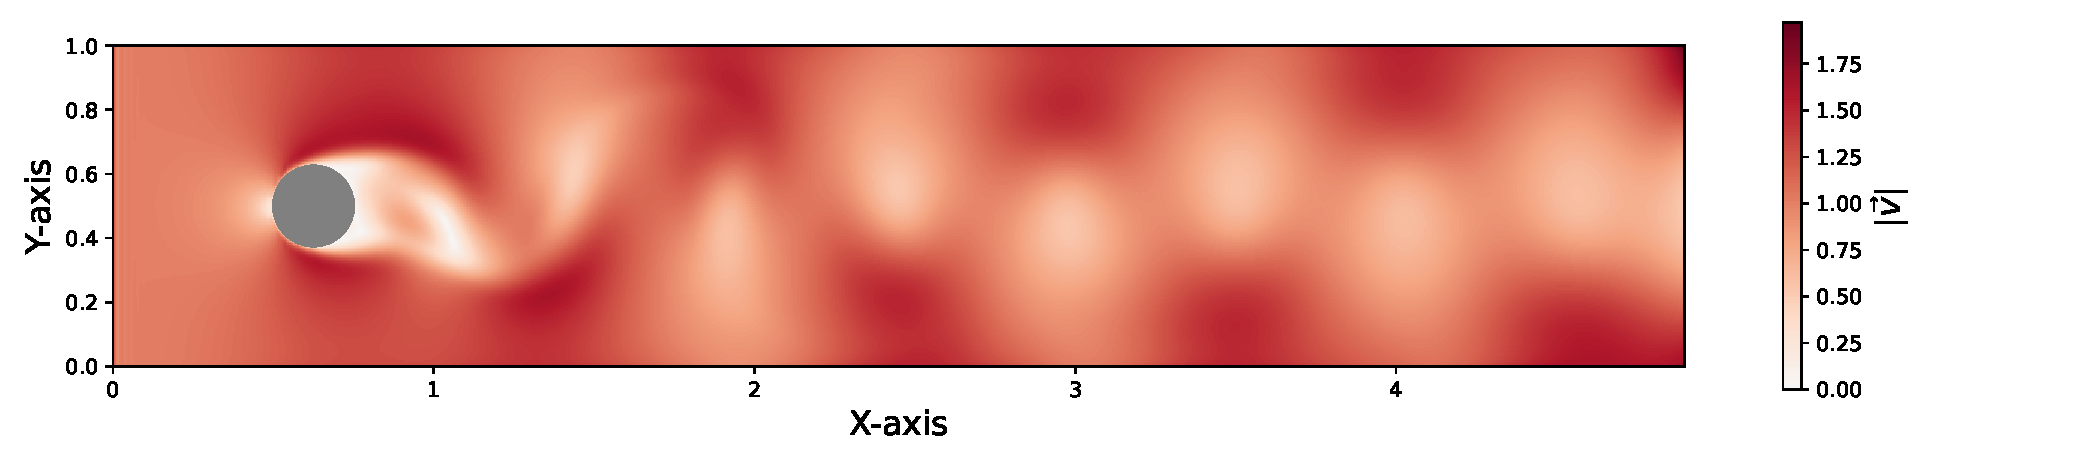
\includegraphics[width=\linewidth]{0_graphics/numeric/absV_25_sim.pdf}
    \caption{Absolute velocity $|\vec{v}|$}
    \label{fig:abs_velocity_25}
  \end{subfigure}
  \vspace{1em} % Adjust space between subfigures as needed
  \hspace*{0.7cm}
  \begin{subfigure}[b]{\linewidth} % Adjust the width as needed
    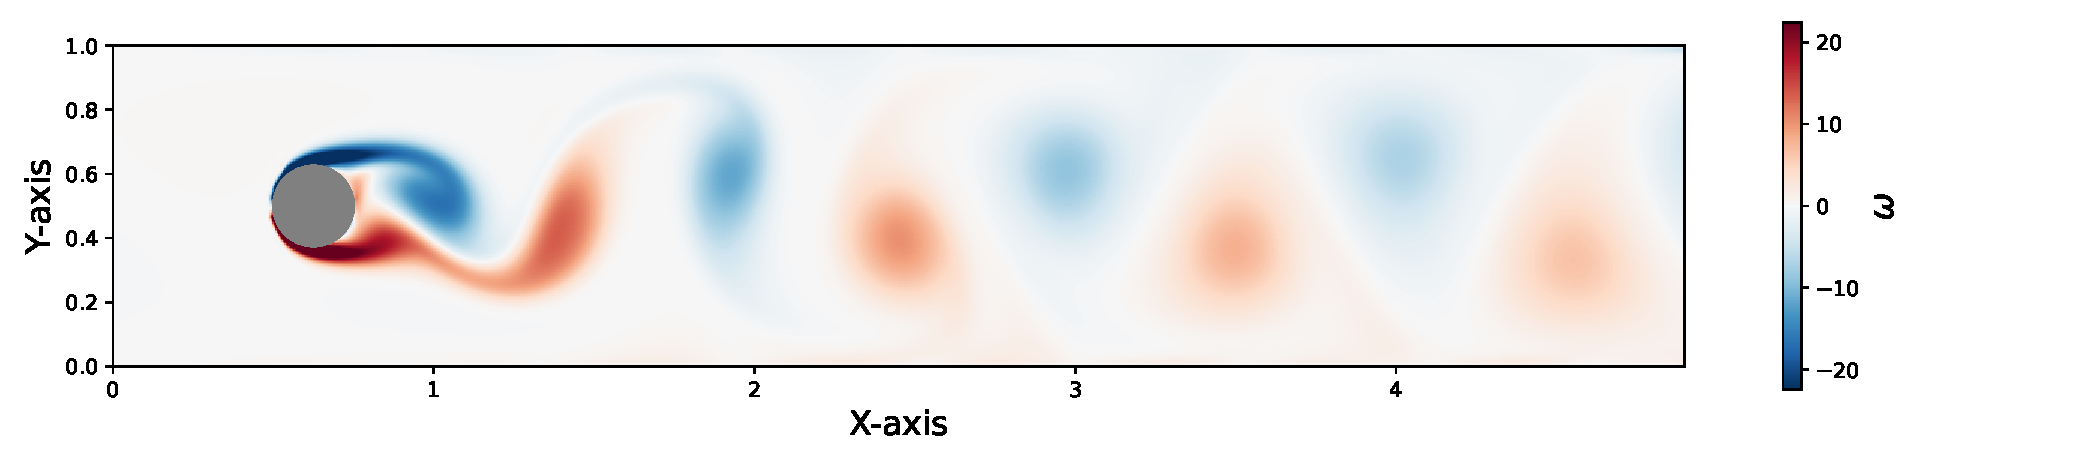
\includegraphics[width=\linewidth]{0_graphics/numeric/vor_25_sim.pdf} % Assuming a different file for vorticity
    \caption{Vorticity $\omega$.}
    \label{fig:vorticity_25}
  \end{subfigure}
  \vspace{-15pt}
  \caption{Flow dynamics around a circular obstacle in a fluid with dynamic viscosity similar to air ($\mu = 1.506 \times 10^{-5}$) at time $t=25$. The top image displays the absolute velocity $|\vec{v}|$, and the bottom image focuses on the vorticity $\omega$.}
  \label{fig:first_karman}
\end{figure}


\subsection{Influence of Reynolds number}
% Analysis how high low reynoldsnumber influence the flow and the phenomenon Maybe there is a limit for our solver or there is a limit for the phenomenon 
The Reynolds number ($\Rey$) plays an important role in determining the flow characteristics around bodies in a fluid. As explained in \cref{sec: posingProblem}, it is a dimensionless quantity that represents the ratio of inertial forces to viscous forces and serves as a key parameter in predicting the transition from laminar to turbulent flow. In this section, the object is the same circle as before and our characteristic length is therefore $L_c = 2  r = 0.25$. Also the dynamical viscosity is set as before to $\mu = 1.506 \times 10^{-5}$. Therefore by varying the Reynolds number we mean to vary the incoming speed on the left side
The impact of the Reynolds number can be categorized in different regimes.



plots to compare different reynolds numbers e.f. frequency of vortexes by taking the average in one column,

show that there is a maximum/ minimum re for observing the phenomen


\subsection{Influence of the object}

Compare two shapes at same reynolds numbers.
%Vary the object size (diameter of the circle) add a ellipse into the flow Find analogy to construction of wings 